% !TEX root = ../main.tex

\section{Results}

% \begin{itemize}
%     \item Methods on how we're doing simulations and results (with simulations and experimental data)
%     \begin{itemize}
%         \item Different SNRs and maybe even use CAPs
%         \item Selection of HRF explained if both use the same but it's different from what's used for simulating.
%         \begin{itemize}
%             \item What happens? For example with gamma for simulating.
%         \end{itemize}
%         \item Selection of regularization parameter
%         \begin{itemize}
%             \item Present with real data on a voxel
%         \end{itemize}
%     \end{itemize}
% \end{itemize}

\subsection{Performance based on the regularization parameter}
\label{sec:regpath}

Figure~\ref{fig:sim}A shows the regularization paths of PFM and TA side by side obtained for the spike model of Eq.~\eqref{eq:pfm_spike} for SNR=3 dB. The solutions for all three SNR conditions are shown in Figures~\ref{fig:path_spike} and \ref{fig:path_block}. Starting from the maximum $\lambda$ corresponding to a null estimate and for decreasing values of $\lambda$, LARS computes a new estimate at the value of $\lambda$ that reduces the sparsity promoted by the \(l_1\)-norm and causes a change in the active set of non-zero coefficients of the estimate (i.e., a zero coefficient becomes non-zero or vice versa) as shown in the horizontal axis of the heatmaps. Vertical dashed lines depict the selection of the regularization parameter based on the BIC, and thus, the colored coefficients indicated by these depict the estimated activity-inducing signal $\mathbf{\hat{{s}}}$. Figure~\ref{fig:sim}B illustrates the resulting estimates of the activity-inducing and activity-related hemodynamic signals when basing the selection of $\lambda$ on the BIC for SNR=3 dB. Given that the regularization paths of both approaches are identical, it can be clearly observed that the BIC-based estimates are identical too for the corresponding $\lambda$. Thus, Figures~\ref{fig:sim}A, \ref{fig:sim}B, \ref{fig:path_spike} and \ref{fig:path_block} demonstrate that, regardless of the simulated SNR condition, the spike model of both deconvolution algorithms produces identical regularization paths when the same HRF and regularization parameters are applied, and hence, identical estimates of the activity-inducing signal $\mathbf{\hat{{s}}}$ and neuronal-related hemodynamic signal $\mathbf{\hat{{x}}}$. Likewise, Figure~\ref{fig:sim}C demonstrates that the regularization paths for the block model defined in Eqs.~\eqref{eq:TA} and~\eqref{eq:pfm_block} also yield virtually identical estimates of the innovation signals for both PFM and TA methods. Again, the BIC-based selection of $\lambda$ is identical for both PFM and TA. As illustrated in Figure~\ref{fig:sim}D, the estimates of the innovation signal $\mathbf{u}$ also show no distinguishable differences between the algorithms. % Hence, Figures~\ref{fig:sim} A-D demonstrate that both PFM and TA yield equivalent regularization paths and estimates of the innovation signal and activity-inducing signal regardless of the simulated SNR condition when applying the same HRF and regularization parameters with the block and spike models.\todo{Last sentence could be skipped and moved to a general conclusion paper in the discussion}

As for selecting $\lambda$ with the MAD criterion defined in Eq.~\eqref{eq:std}, Figure~\ref{fig:sim}E depicts the estimated activity-inducing and activity-related signals for the simulated low-SNR setting using the spike model, while Figure~\ref{fig:sim}F shows the estimated signals corresponding to the block model. Both plots in Figure~\ref{fig:sim}E and F depict nearly identical results between PFM and TA with both models. Given that the regularization paths of both techniques are identical, minor dissimilarities are owing to the slight differences in the selection of $\lambda$ due to the quantization of the values returned by LARS.

\begin{figure}[t!]
    \begin{center}
        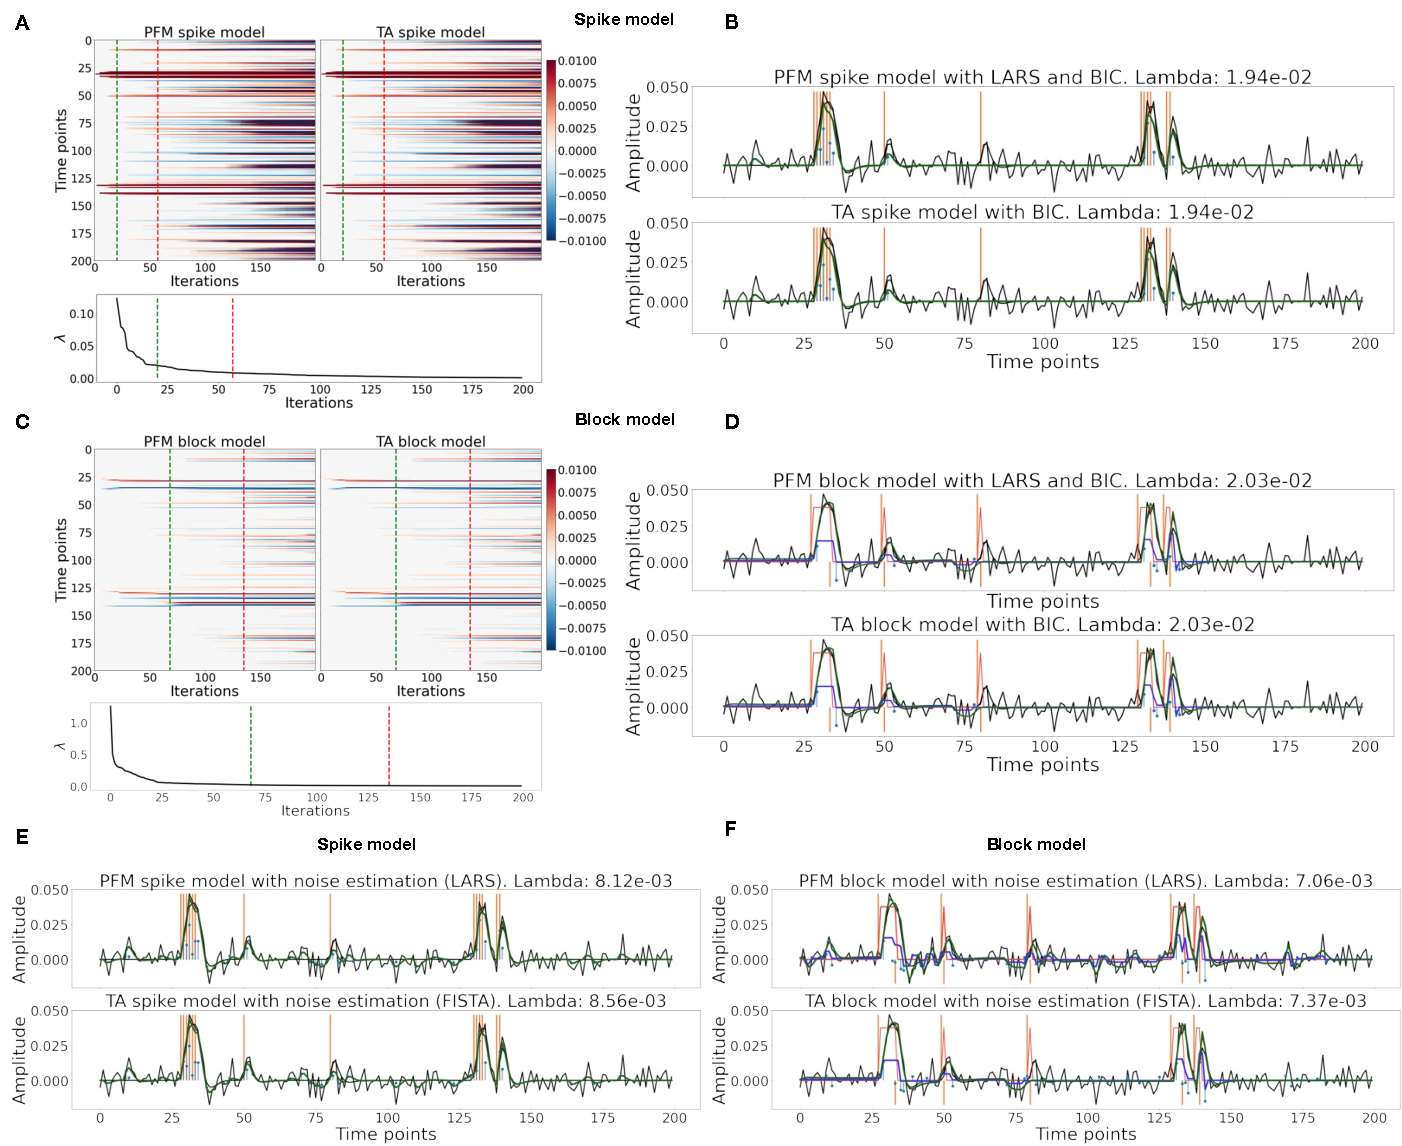
\includegraphics[width=\textwidth]{figures/figure_sim.pdf}
    \end{center}
    \caption{(A) Heatmap of the regularization paths of the activity-inducing signals (spike model) estimated with PFM and TA as a function of $\lambda$ for the simulated data with SNR = 3 dB (x-axis: increasing number of iterations or $\lambda$ as given by LARS; y-axis: time; color: amplitude). Vertical lines denote iterations corresponding to the BIC (dashed line) and MAD (dotted line) selection of $\lambda$. (B) Estimated activity-inducing (blue) and activity-related (green) signals with a selection of $\lambda$ based on the BIC. Orange and red lines depict the ground truth. (C) Heatmap of the regularization paths of the innovation signals (block model) estimated with PFM and TA as a function of $\lambda$ for the simulated data with SNR = 3 dB. (D) Estimated innovation (blue), activity-inducing (darker blue), and activity-related (green) signals with a selection of $\lambda$ based on the BIC. (E) Activity-inducing and activity-related (fit, $\mathbf{x}$) signals estimated with PFM (top) and TA (bottom) when $\lambda$ is selected based on the MAD method with the spike model, and (F) with the block model for the simulated data with SNR = 3 dB.}
\label{fig:sim}
\end{figure}

% Furthermore, we performed the same analysis on experimental data as shown in Figure~\ref{fig:exp} (rows 1-2, 4). Row 1 demonstrates that the PFM and TA regularization paths are identical when deconvolving experimental data, regardless of the deconvolution model (spike or block). Even though tiny differences can be seen between the two methods in the BIC selection of \(\lambda\) in row 4, row 2 proves that the results are practically identical, and differences can be disregarded.

\subsection{Performance on experimental data}

\todo{Just a thought: wouldn't the range of values be easier to assess if we take the square root of the SSD? Like an STD in the end? The fact that these values are ``negligible'' can only be grasped if you give an estimate too of the range of typical signal excursions.}
Figure~\ref{fig:rss} depicts the SSD maps revealing differences between PFM and TA estimates for the spike (Figure~\ref{fig:rss}A and C) and block (Figure~\ref{fig:rss}B and D) models when applied to the three experimental fMRI datasets. The SSD values are virtually negligible (i.e., depicted in yellow) in most of the within-brain voxels and clearly lower than the amplitude of the estimates of the activity-inducing and innovation signals. Based on the maximum value of the range shown in each image, we observe that the similarity between both approaches is more evident for the spike model (with both selection criteria) and the block model with the BIC selection. However, a selection of the regularization parameter $\lambda$ based on the MAD estimate of the noise using the block model produces higher\todo{Again, higher, but without ``calibration'' is difficult.} SSD values, with the largest differences occurring in gray matter voxels. These areas also correspond to low values of $\lambda$ (see Figure~\ref{fig:lambdas}) and MAD estimates of the noise (see Figure~\ref{fig:mad_estimate}), while the highest values are visible in regions with signal droupouts, ventricles, and white matter.

\begin{figure}[t!]
    \begin{center}
        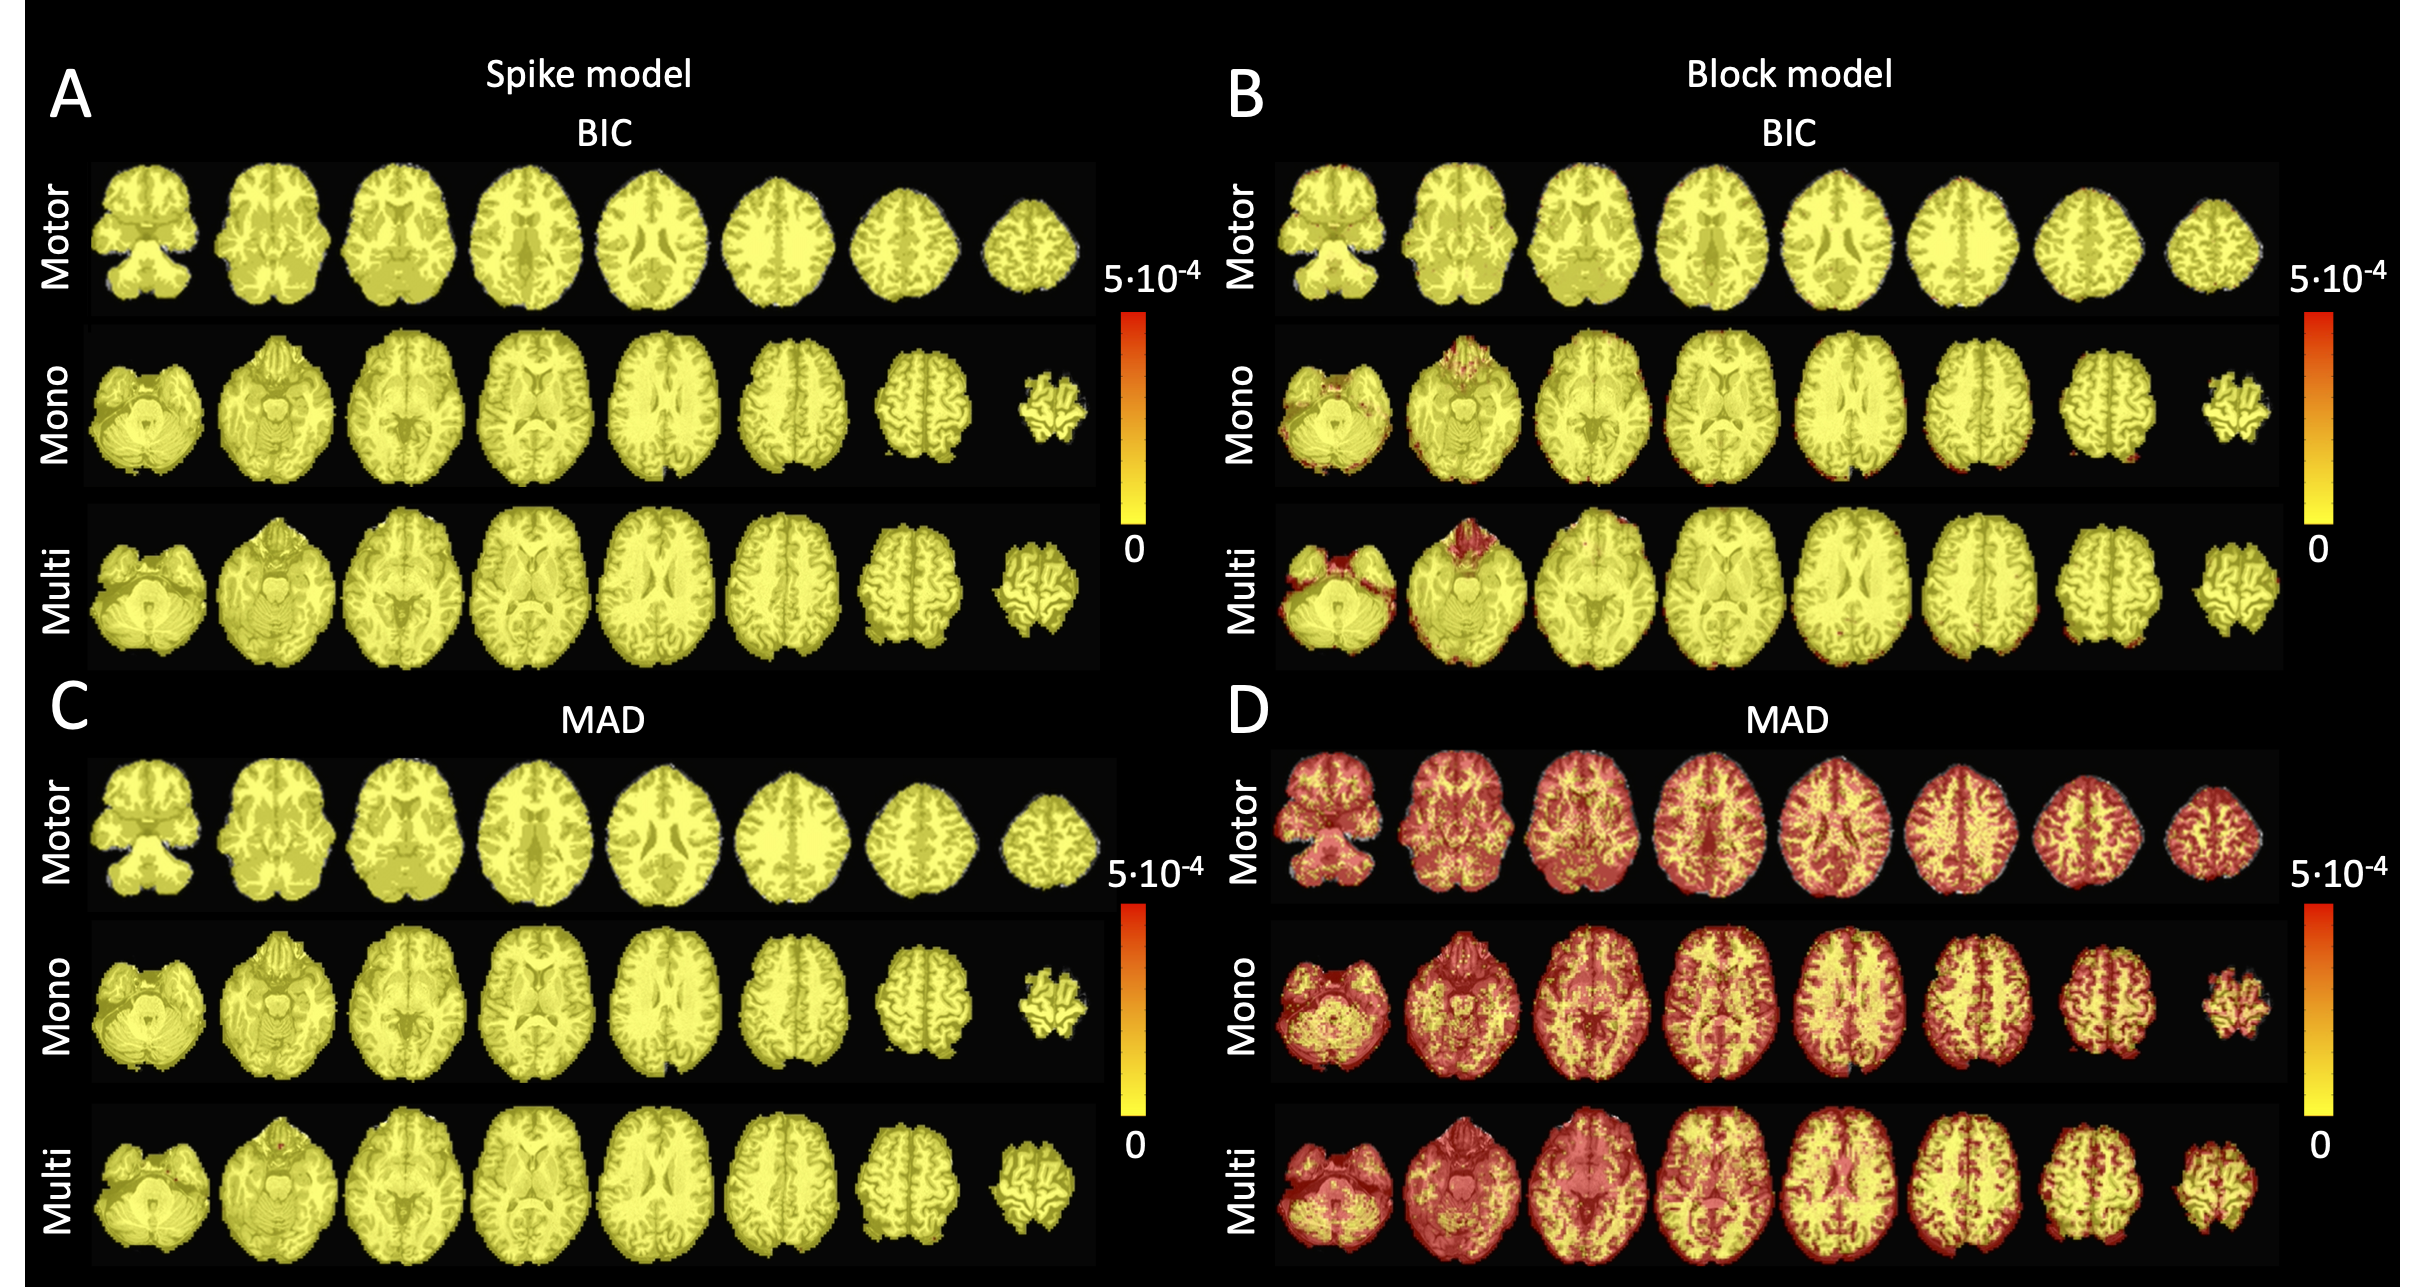
\includegraphics[width=\textwidth]{figures/comp_figure.png}
    \end{center}
    \caption{Sum of squared differences (SSD) between the estimates obtained with PFM and TA for (A) spike model (activity-inducing signal) and BIC selection of $\lambda$, (B) block model (innovation signal) and BIC selection, (C) spike model (activity-inducing signal) and MAD selection, (D) block model (innovation signal) and MAD selection. SSD maps are shown for the three experimental fMRI datasets: the motor task (Motor), the monoband resting-state (Mono), and the multiband resting-state (Multi) datasets.}
\label{fig:rss}
\end{figure}

Figure~\ref{fig:task_maps} depicts the results of the analysis of the Motor dataset with the PFM and TA algorithms using the BIC selection of $\lambda$ (see Figure~\ref{fig:task_mad} for results with MAD selection), as well as a conventional GLM approach. The Activation Time Series (top left), calculated as the sum of squares of all voxel amplitudes (positive vs. negative) for a given moment in time, obtained with PFM and TA show nearly identical patterns. These ATS help to summarize the four dimensional information available in the results across the spatial domain and identify instances of significant BOLD activity. The second to sixth rows show the voxel timeseries and the corresponding activity-related, activity-inducing and innovation signals obtained with PFM using the BIC criterion of representative voxels in the regions activated in each of the motor tasks. The TA-estimated time-series are not shown because they were virtually identical. The maps shown on the right correspond to statistical parametric maps obtained with the GLM for each motor condition ($p < 0.001$) as well as the maps of the PFM and TA estimates at the onsets of individual motor events (indicated with arrows in the timecourses). The estimated activity-related, activity-inducing and innovation signals clearly reveal the activity patterns of each condition in the task, as they exhibit a BOLD response locked to the onset and duration of the conditions. Overall, activity maps of the innovation signal obtained with PFM and TA highly resemble those obtained with a GLM for individual events.

Notice that the differences observed with the block model and a selection of $\lambda$ based on the MAD estimate shown in Figure~\ref{fig:rss} are reflected on the ATS shown in Figure~\ref{fig:task_mad}. Returning to Figure~\ref{fig:task_maps}, 

\todo[inline]{I am a bit puzzled by the ranges of values... so SSD is up to $10^{-4}$, but the (signed) SSD values in first row of Fig.~5 happily range up to 50, quite high if their average should drop below $10^{-4}$? Then, on the ATS, the range is rather $0-0.10$, which is very low again compared to SSDs in the range of $10-50$. Finally, the maps on the right-hand side are selected from timepoints that have values in the range $0.05-0.10$, but the map seems saturated (?) at $10^{-3}$.}

\begin{figure}[t!]
    \begin{center}
        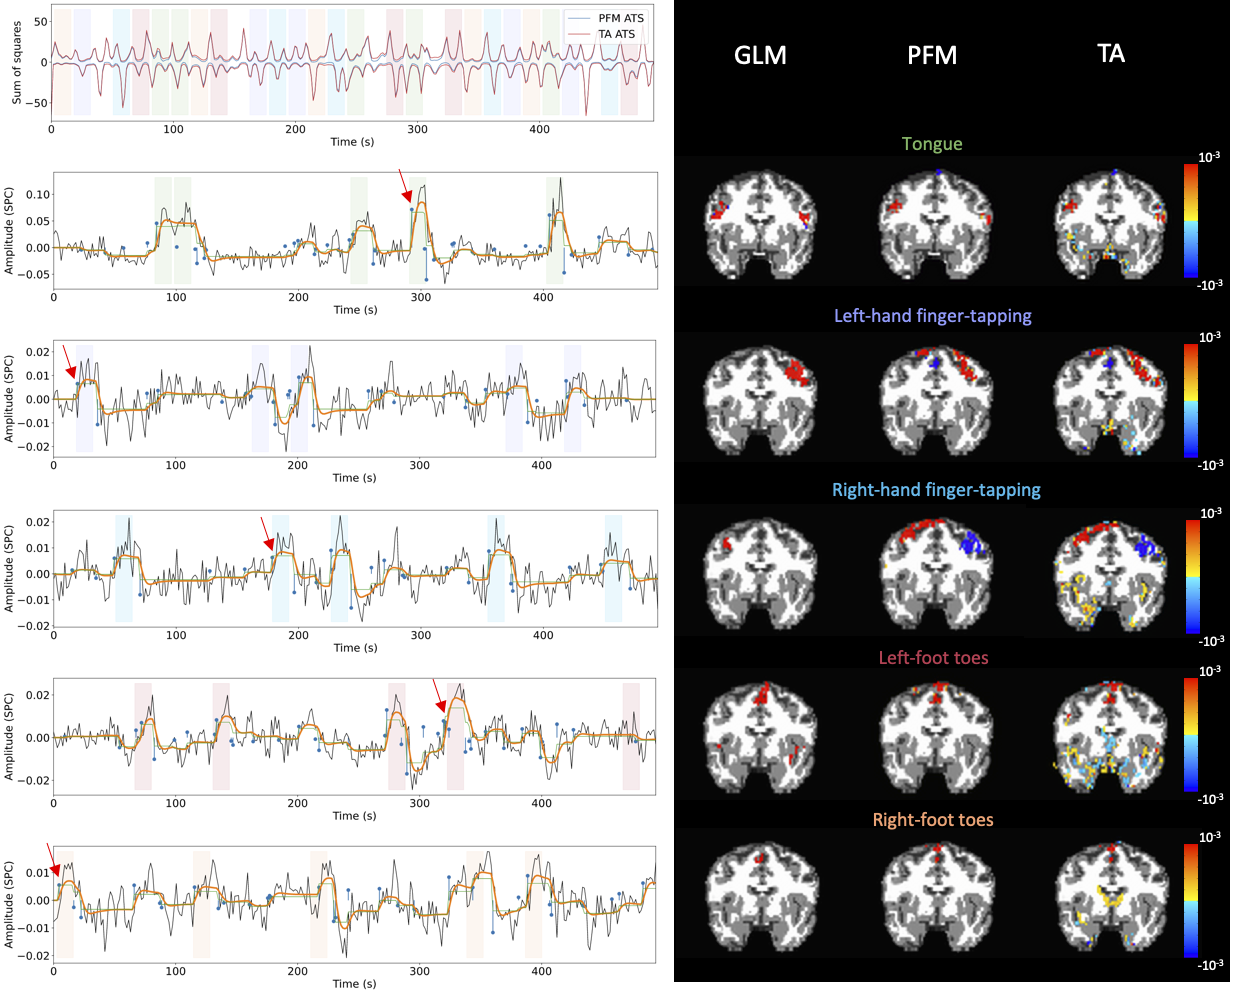
\includegraphics[width=\textwidth]{figures/task_maps.png}
    \end{center}
    \caption{Activity maps of the motor task using a selection of $\lambda$ based on the BIC estimate. Row 1: Activation time-series (ATS) of the innovation signals estimated by PFM (in blue) or TA (in red) calculated as the sum of squares of all voxels at every timepoint. Positive-valued and negative-valued contributions were separated into two distinct time-courses. Color-bands indicate the onset and duration of each condition in the task (green: tongue motion, purple: left-hand finger-tapping, blue: right-hand finger-tapping, red: left-foot toes motion, orange: right-foot toes motion). Rows 2-6: time-series of a representative voxel for each task with the PFM-estimated innovation (blue), PFM-estimated activity-inducing (green), and activity-related (i.e., fitted, orange) signals, with their corresponding GLM, PFM, and TA maps on the right (representative voxels indicated with green arrows). Amplitudes are given in signal percentage change (SPC). The maps shown on the right are sampled at the time-points labeled with the red arrows and display the innovation signals at these moments across the whole brain.}
\label{fig:task_maps}
\end{figure}

As an illustration of the insights that deconvolution methods can provide in the analysis of resting-state data, Figure~\ref{fig:caps} depicts the CAPs and iCAPs obtained from thresholding and averaging the activity-inducing and innovation signals, respectively, estimated from the resting-state multiband data using PFM with a selection of $\lambda$ based on the BIC. The activity-inducing CAPs obtained via deconvolution show spatial patterns of the default mode network (DMN), dorsal attention network (DAN) and visual network (VIS) that highly resemble the maps obtained with conventional seed correlation analysis using Pearson's correlation, and the CAPs based on the amplitude of the signal (i.e., with no deconvolution). With deconvolution, the CAPs seem to depict less spurious voxels (mainly negative) and more accurate spatial delineation (i.e., less smoothness) than those obtained from the original data, while mantaining the structure of the networks. The BIC-informed selection of $\lambda$ yields spatial patterns of CAPs and iCAPs that are more sparse than those obtained with a selection of $\lambda$ based on the MAD estimate (see Figure~\ref{fig:caps_mad}). Furthermore, the spatial patterns of the iCAPs based on the innovation signals using the block model yield complementary information to those obtained with the activity-inducing signal since iCAPs allow to reveal regions with synchronous innovations, i.e., with the same upregulating and downregulating events. For instance, it is interesting to observe that the structure of the visual network nearly disappears in its corresponding iCAP, suggesting the existence of different temporal neuronal patterns across voxels in the primary and secondary visual cortices. 

\begin{figure}[t!]
    \begin{center}
        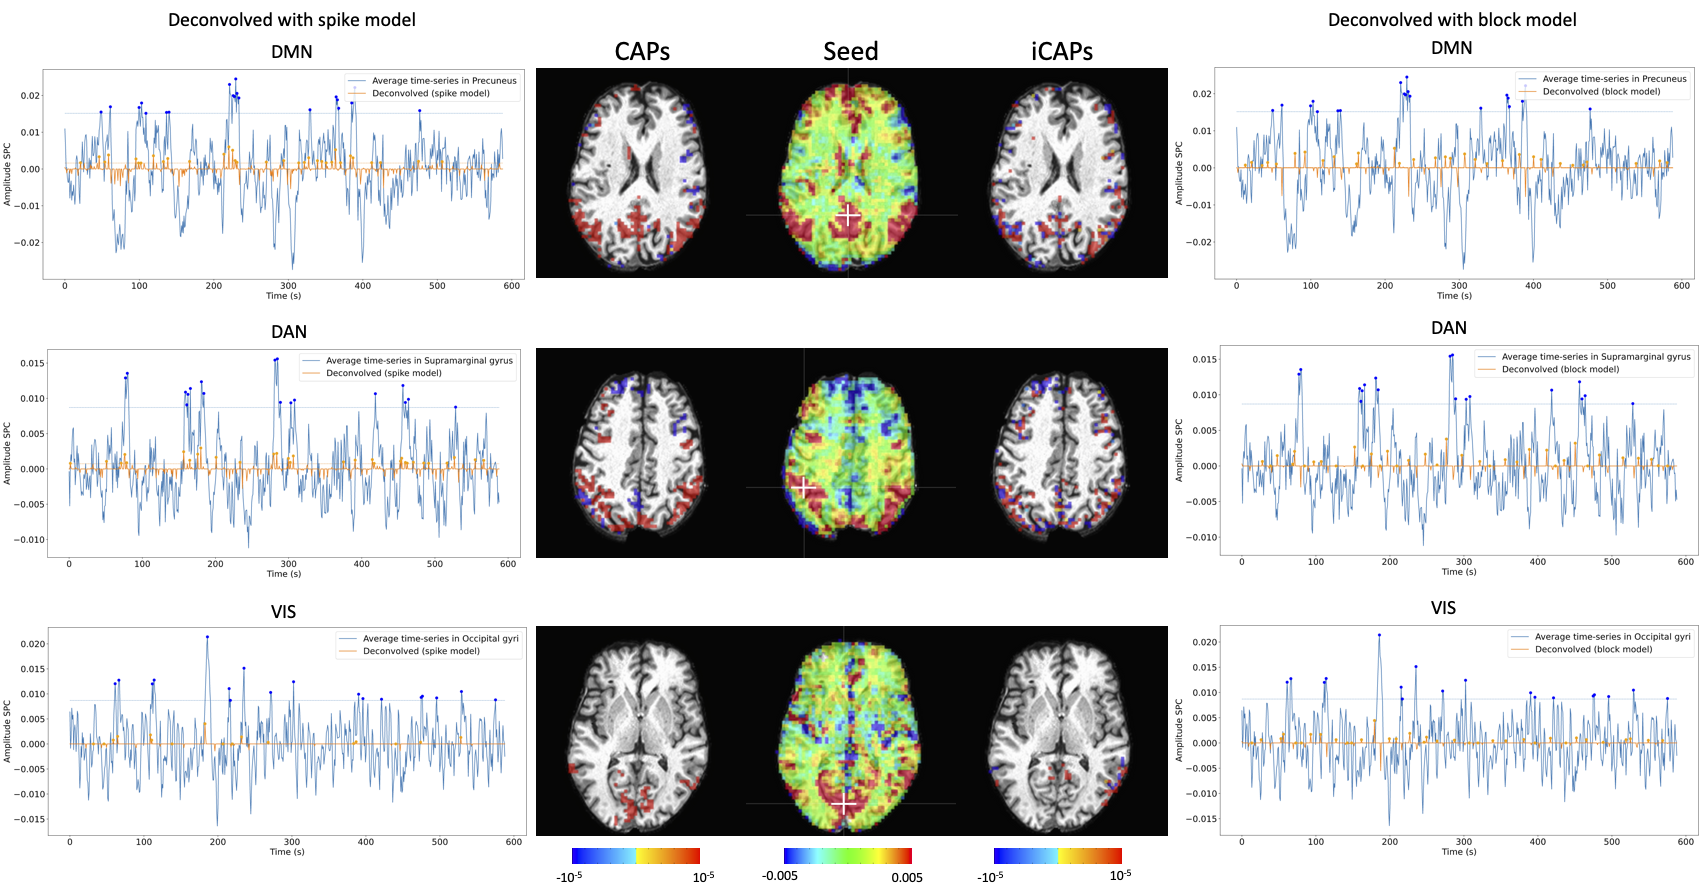
\includegraphics[width=\textwidth]{figures/caps.png}
    \end{center}
    \caption{Activity-inducing co-activation patterns (activity-inducing CAPs, left) and innovation-driven co-activation patterns (innovation CAPs, right) obtained from PFM-estimated activity-inducing and innovation signals, respectively, using a BIC-based selection of $\lambda$. Time-points selected with a 95\textsuperscript{th} percentile threshold (horizontal lines) are shown over the average time-series (blue) in the seed region (white cross) and the deconvolved signals, i.e., activity inducing (left) and innovation (right) signals (orange). CAPs and seed correlation maps are illustrated in the center.}
\label{fig:caps}
\end{figure}